\title{Solid State Physics: Final Exam Review}
\date{\today}

\documentclass[10pt]{article}
\usepackage{amsthm}
\usepackage{subcaption}
\usepackage{listings}
\usepackage{graphicx}
\usepackage{physics}

\graphicspath{ {figures/} }
\begin{document}
\maketitle

\section{LCAO and Tight Binding}
\subsection{Gentle Introduction: Covalent Bonding of Hydrogen Atoms}
Imagine a system in which two Hydrogen atoms are held with fixed-position nuclei
("Born-Oppenheimer Approximation") and a shared electron between them.
Goal: calculate the eigenenergies of the system as a funtion of the distance from the fixed nuclei.


The Hamiltonian of the system is given by

$$
H = K + V_{1} + V_{2}
$$

where
$$
K = \frac{\textbf{p}^{2}}{2m}
$$
and the coulombic potential due to the nucleus fixed at position $\textbf{R}_{i}$ is given by
$$
V_{i} = \frac{e^{2}}{4\pi\epsilon_{0}|\textbf{r} - \textbf{R}_{i}|}
$$
We can write down a trial solution of the form
$$
\ket{\psi} = \phi_{1}\ket{1} + \phi_{2}\ket{2}
$$
where $\ket{i}$ are the atomic orbitals (or ``tight-binding orbitals'') representing the
ground state solution for that particular isolated nucleus. That explicitly means the following
$$
(K + V_{1})\ket{1} = \epsilon_{0}\ket{1}
$$
$$
(K + V_{2})\ket{2} = \epsilon_{0}\ket{2}
$$
where $\epsilon_{0}$ is the ground state energy of a single Hydrogen atom.

In the LCAO/tight-binding method, we make the following approximation: \textbf{the
atomic orbitals $\ket{i}$ are orthogonal} such that
$$
\bra{i}\ket{j} = \delta_{ij}
$$
The Schrodinger equation can be written as
$$
H\ket{\psi} = E\ket{\psi}
$$
or, alternatively, in the $\ket{i}$ basis:
$$
\begin{bmatrix}
  H_{11} & H_{12} \\
  H_{21} & H_{22}
\end{bmatrix}
\begin{bmatrix}
  \phi_{1} \\
  \phi_{2}
\end{bmatrix}
 = E \begin{bmatrix}
   \phi_{1} \\
   \phi_{2}
 \end{bmatrix}
$$
By using a variational method where
$$
E = \frac{\bra{\psi}H\ket{\psi}}{\bra{\psi}\ket{\psi}}
$$
and
$$
\frac{\partial E}{\partial \phi_{i}} = \frac{\partial E}{\partial \phi_{i}*} = 0
$$
We obtain an eigenvalue equation
$$
\sum_{j}H_{ij}\phi_{j} = E\phi_{i}
$$
where $H_{ij} = \bra{i}H\ket{j}$. The components of $H$ can be written explicitly as
$$
H_{11} = \bra{1}H\ket{1} = \bra{1}K+V_{1}\ket{1} + \bra{1}V_{2}\ket{1} = \epsilon_{0} + V_{cross}
$$
$$
H_{22} = \bra{2}H\ket{2} = \bra{2}K+V_{2}\ket{2} + \bra{2}V_{1}\ket{2} = \epsilon_{0} + V_{cross}
$$$$
H_{12} = \bra{1}H\ket{2} = \bra{1}K+V_{2}\ket{2} + \bra{1}V_{1}\ket{2} = -t
$$$$
H_{21} = \bra{2}H\ket{1} = \bra{2}K+V_{1}\ket{1} + \bra{2}V_{2}\ket{1} = -t^*
$$
We make the following observations:
\begin{itemize}
  \item The on-site energy is given by
  $$\bra{i}K + V_{i}\ket{i} = \epsilon_{0}$$
  \item The coulombic potential due to site $j$ on site $i$ is given by
  $$\bra{i}V_{j}\ket{i} = V_{cross}$$
  \item The \emph{hopping term} is defined by
  $$\bra{j}V_{j}\ket{i} = \bra{i}V_{i}\ket{j}^* = -t$$
\end{itemize}

The eigenvalue equation then takes on the form of a $2\times 2$ matrix equation
$$
\begin{bmatrix}
  \epsilon_{0} + V_{cross} & -t \\
  -t^{*} & \epsilon_{0} + V_{cross}
\end{bmatrix}
\begin{bmatrix}
  \phi_{1} \\
  \phi_{2}
\end{bmatrix}
= E\begin{bmatrix} \phi_{1} \\ \phi_{2} \end{bmatrix}
$$
Diagonalization yields the eigenenergies
$$
E_{\pm} = \epsilon_{0} + V_{cross} \pm |t|$$

\subsection{Tight-Binding Chain}
In this section, we seek to observe that all waves in periodic environments behave similarly. Here
we consider electron waves, but we should consider the similarities to vibrational waves (phonons) as
well.

The one-dimensional tight binding has the following description.
\begin{itemize}
  \item There is a single orbital on atom $n$, denoted $\ket{n}$.
  \item Periodic boundary conditions are imposed such that $\ket{N} = \ket{0}$.
  \item Atomic orbital states are orthogonal.
  $$\bra{n}\ket{m} = \delta_{nm}$$
  \item The general trial wavefunction has the form
  $$\ket{\Psi} = \sum_{n}\phi_{n}\ket{n}$$
  \item The effective Schrodinger equation is
  $$
  \sum_{m}H_{nm}\phi_{m} = E\phi_{n}
  $$
  where $H_{nm} = \bra{n}H\ket{m}$.
  \item The Hamiltonian can be written
  $$
  H = K + \sum_{j}V_{j}
  $$
  where $K = \textbf{p}^{2}/2m$ and $V_{j} = V(\textbf{r} - \textbf{R}_{j})$.
\end{itemize}
Given the description above, we have
\begin{equation}
\begin{aligned}
  H\ket{m} & = (K + V_{m})\ket{m} + \sum_{j \neq m}V_{j}\ket{m} \\
           & = \epsilon_{atomic}\ket{m} + \sum_{j \neq m}V_{j}\ket{m}
\end{aligned}
\end{equation}
Therefore,
$$
H_{nm} = \bra{n}H\ket{m} = \epsilon_{atomic}\delta_{mn} + \sum_{j \neq m}\bra{n}V_{j}\ket{m}
$$
where
$$
\sum_{j \neq m}\bra{n}V_{j}\ket{m} = \left\{\begin{matrix}
 V_{0} & n=m \\
 -t & n=m\pm 1\\
 0 & 0
\end{matrix}\right.
$$
So,
$$
H_{n,m} = (\epsilon_{atomic} + V_{0})\delta_{nm} -t(\delta_{n+1,m} + \delta_{n-1,m}) = \epsilon_{0}\delta_{nm} -t(\delta_{n+1,m} + \delta_{n-1,m})
$$

\subsubsection{Solution}
We propose an ansatz
$$\phi_{n} = \frac{e^{-ikna}}{\sqrt{N}}$$
Note the absence of of a frequency component to the exponent, which is due
to the fact that we are seeking solutions to the time-independent Schrodinger
equation.
\begin{itemize}
  \item For a system with $N$ sites, and length $L = Na$, there are $N$ possible
  solutions of the ansatz form.
  \item Each solution corresponds to $k = 2\pi m/L$, where $m = 0, ..., N-1$.
\end{itemize}
Plugging the ansatz into the Schrodinger equation gives
\begin{equation}
\sum_{m}H_{nm}\phi_{m} = \epsilon_{0}\frac{e^{-ikna}}{\sqrt{N}} - t\left( \frac{e^{-ik(n+1)a}}{\sqrt{N}} + \frac{e^{-ik(n-1)a}}{\sqrt{N}}\right)
\end{equation}
and we also know that
\begin{equation}
  E\phi_{n} = E\frac{e^{-ikna}}{\sqrt{N}}
\end{equation}
Equating the previous two equations gives us
$$
E = \epsilon_{0} - 2t\cos(ka)
$$
(Note the correspondance to the phonon spectrum for the 1D monatomic chain). The dispersion curve is shown in Fig. 1.

\begin{figure}
  \centering
    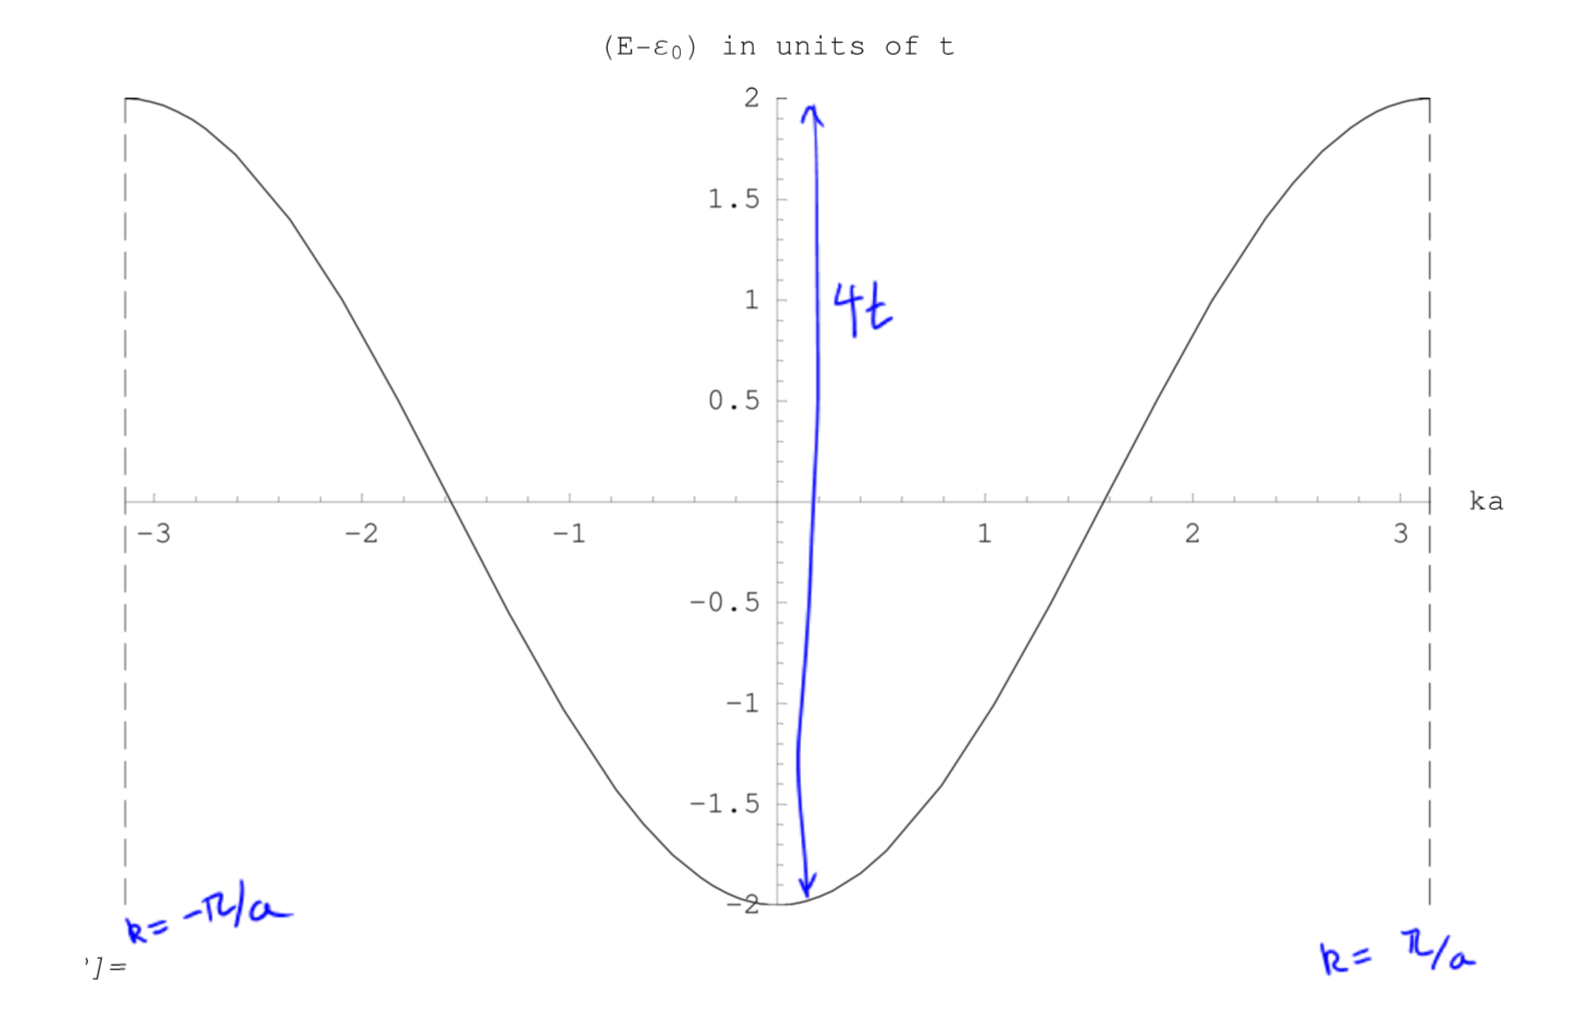
\includegraphics[width=\textwidth]{tb1}
    \caption{Dispersion curve for tight-binding chain.}
\end{figure}

Some notes about the dispersion relation:
\begin{itemize}
  \item The periodicity is $k \rightarrow k + \frac{2\pi}{a}$ (like phonons).
  \item Zero group velocity (flat curve) at the Brillouin zone boundary (like phonons).
  \item Electrons may only have eigenstates within a certain \emph{band}, referring to both
  the energy range in which the eigenstates exist as well as the individual branches
  of the dispersion curve itself.
  \item The \emph{bandwidth} refers to the difference between the maximum and minimum energies
  in a band. In Fig. 1, the bandwidth is $4t$.
  \item The bandwidth, $4t$, is dependent on the hopping amplitude and, therefore, on the
  interatomic spacing between nuclei. This dependence is shown in Fig. 2.
  \item As seen in Fig. 2, the effect of the hopping is to raise the energy of some eigenstates and lower the
  energy of others (such that the average is still $\epsilon_{0}$). If the band is not completely filled, then
  the average energy dips below $\epsilon_{0}$ since some higher states are not filled.
\end{itemize}

\begin{figure}
  \centering
    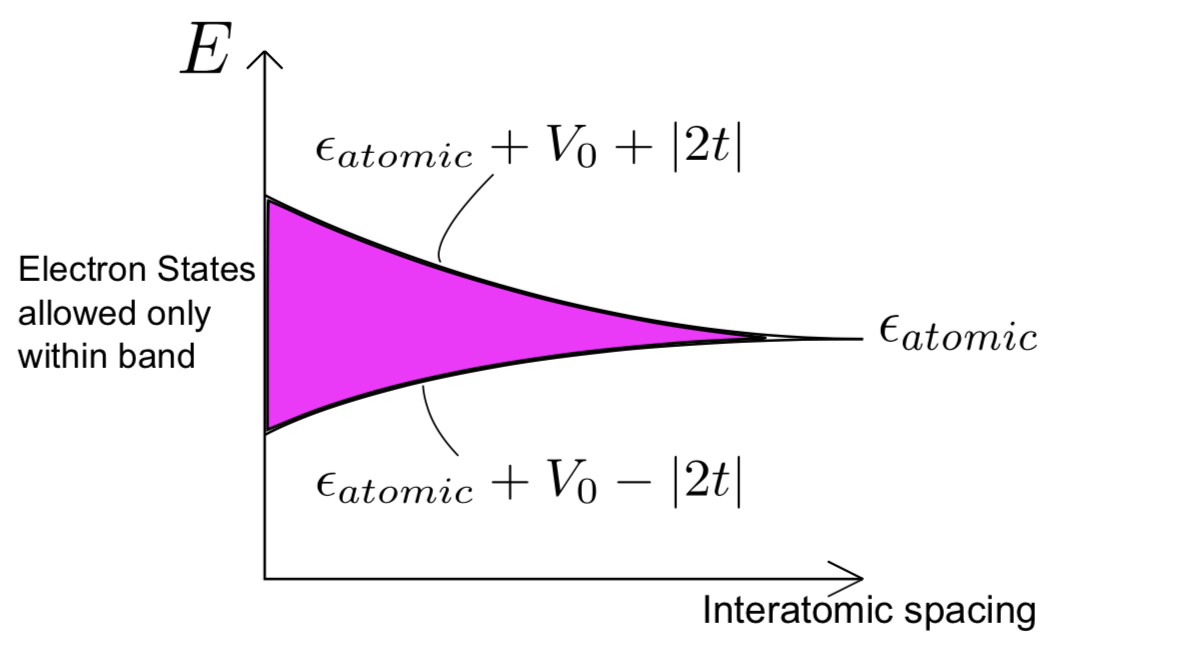
\includegraphics[width=\textwidth]{tb2}
    \caption{Bandwidth dependence on interatomic spacing.}
\end{figure}

Near the bottom of the band in Fig. 1, where $k$ is close to zero, the dispersion is approximately parabolic. For
small $k$, $cos(ka) \approx 1 - k^{2}a^{2}/2$, so

$$
E(k) \approx Constant + ta^{2}k^{2}
$$

\textbf{Note:} If the minimum were at the Brillouin zone edge, we would need to expand around $k = \pi/a$ instead.
Since the dispersion of the free electron can be written as
$$E_{free}(k) = \frac{\hbar^{2}k^{2}}{2m}$$
We can relate the two dispersion relations to calculate an \emph{effective mass} $m^{*}$ such that the dispersion at
the bottom of the band behaves as a free electron of mass $m^{*}$.
$$
\frac{\hbar^{2}k^{2}}{2m^{*}} = fa^{2}k^{2}
$$
and the effective mass is then
$$
m^{*} = \frac{\hbar^{2}}{2ta^{2}}
$$

\subsection{Band Filling}
\subsubsection{Monovalent Case}
If every atom in the one-dimensional, single-orbital tight binding model were to ``donate'' an electron,
then we would have a total of $N$ electrons. These electrons occupy the $N$ lowest-energy states in the band,
which has $N$ allowed eigenstates, but each eigenstate can be populated by a spin-up and a spin-down electron.
The band is therefore only half filled, as seen in the left of Fig. 3.

In Fig. 3, the Fermi surface (the energy level separating occupied and unoccupied states) is $\epsilon_{0}$. By providing a small bit of
energy, the Fermi sea can be shifted slightly such that the electrons take on an average net positive momentum (right side of Fig. 3) and
current is able to flow. For this reason, monovalent materials are frequently metals.

\begin{figure}
  \centering
    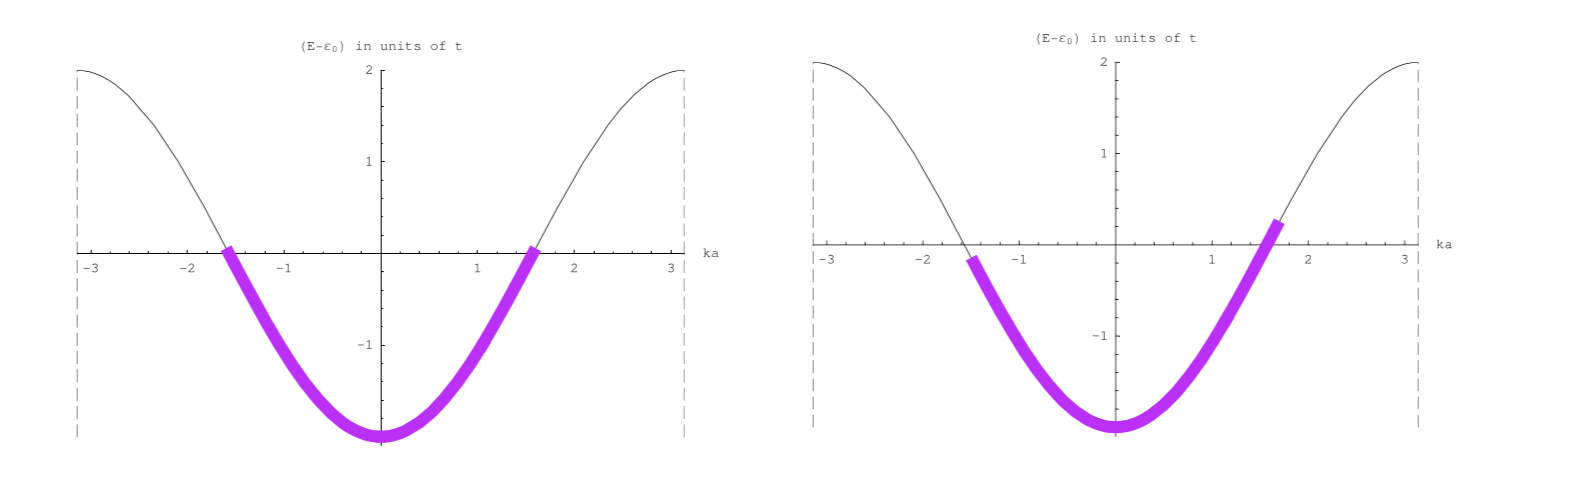
\includegraphics[width=\textwidth]{tb3}
    \caption{Monovalent Fermi surface and shifted Fermi sea.}
\end{figure}

\subsubsection{Divalent Case}
In the divalent case, there are a total of $2N$ atoms, which fill all spin-up and spin-down states of each of the $N$ allowed
eigenstates. That is, the band is completely filled. Therefore, there are no free $k$ states to which the Fermi sea could shift to allow a current to
be induced. \textbf{A filled band carries no current}. This results in a \emph{band insulator}.

\subsection{Multiple Bands}
In the one-dimensional, single-orbital tight-binding model, there is a single band. However, if we consider multiple
orbitals per unit cell, more bands will emerge. We may consider, for example:
\begin{itemize}
  \item Multi-atom unit cells with one or more orbitals each.
  \item Single-site unit cells with multiple orbitals per site.
\end{itemize}
The energy bandwidth as a function of inter-atomic spacing is shown in Fig. 4 for the case where there are two orbitals per single-site.
\begin{figure}
  \centering
    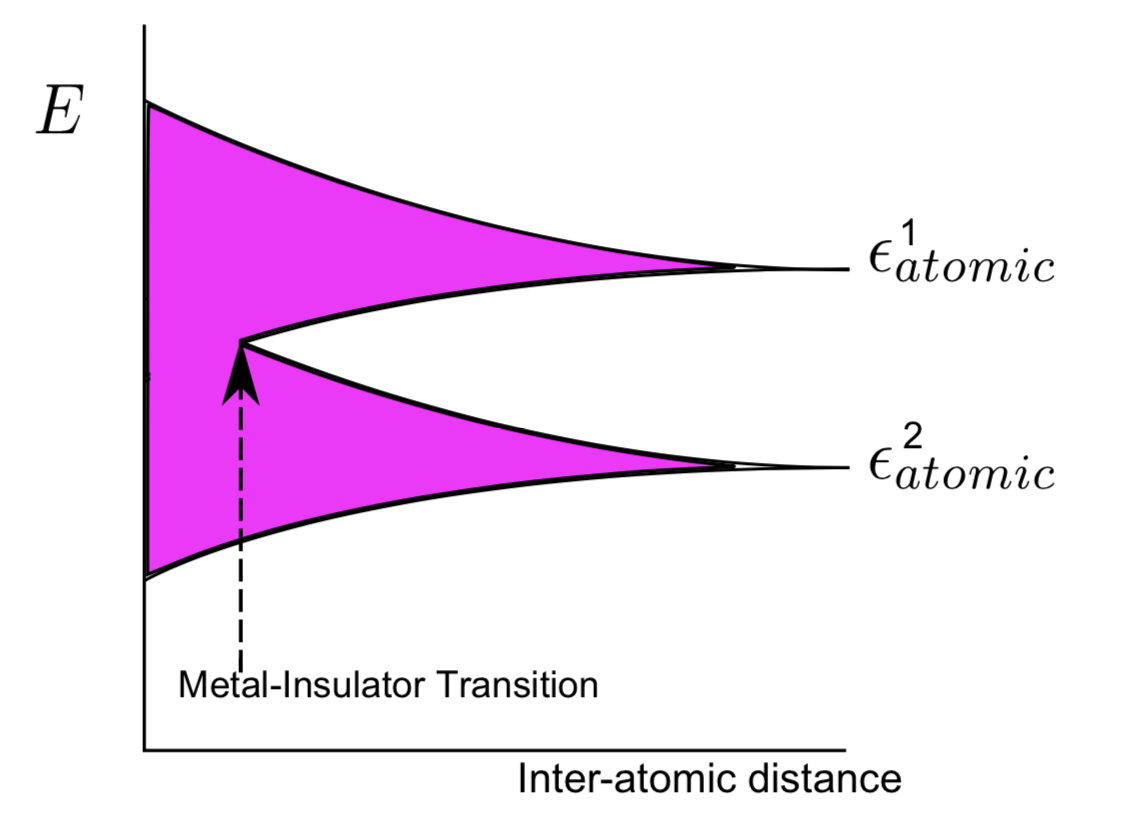
\includegraphics[width=\textwidth]{tb4}
    \caption{Energy bandwidth as a function of inter-atomic distance. Two atomic orbitals per site.}
\end{figure}
The dispersion relation for the two-site, single orbital case is shown in Fig. 5. Some notes:
\begin{itemize}
  \item If both species are divalent, then there are already a total of two electrons filled each orbital on every atom - that is,
  both branches of the dispersion are filled.
  \item If both species are monovalent, then only the bottom band is filled (i.e. only half the states are filled). So, there are $k$
  states available to shift the Fermi sea (around the Fermi surface, which is halfway between the top and bottom bands). However, to
  shift the sea, we need to apply an electric field strong enough to overcome the energy gap between the bands. \textbf{A filled band
  is an insulator as long as there is a finite gap to any higher-level band}.
  \item As seen in Fig. 4, as the interatomic distance decreases, the bandwidths of the individual bands come to overlap and there is no
  longer a gap between the lower- and higher-energy bands. In this limit, the material comes to behave as a metal.
\end{itemize}
\begin{figure}
  \centering
    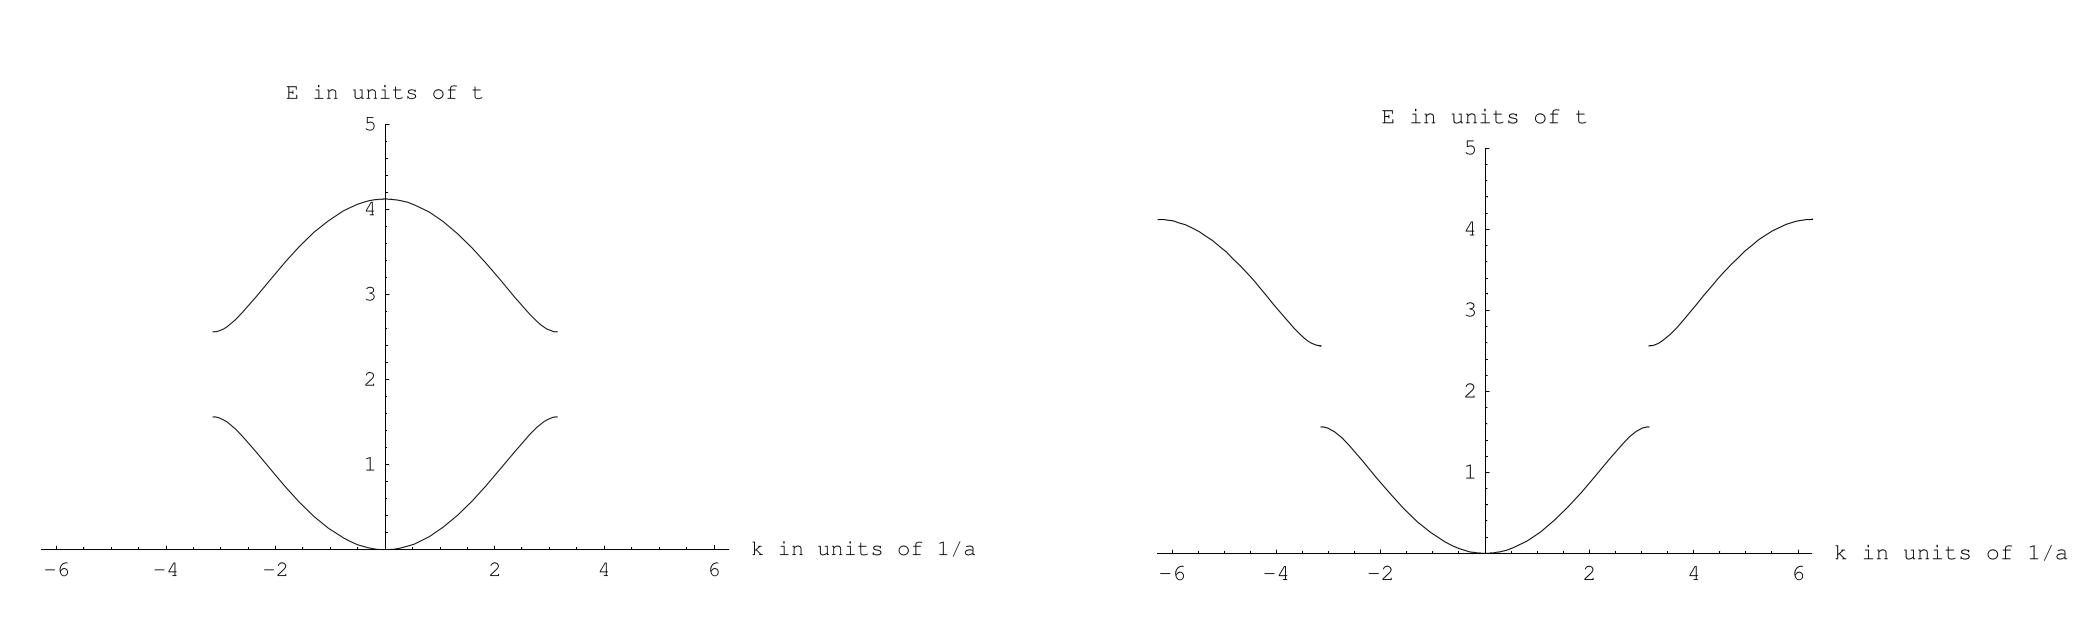
\includegraphics[width=\textwidth]{tb5}
    \caption{Dispersion relation for tight-binding model with two sites per unit cell, one orbital per site.}
\end{figure}

\section{Nearly Free Electron Model}
The difference between the nearly free electron model and the tight binding model:
\begin{itemize}
  \item In the nearly free electron model, electrons are considered as free electron waves that are only very
  weakly perturbed by the periodic potential of the atoms in the solid.
  \item In the tight binding model, electrons are considered very tightly bound to atoms with a possible weak
  hopping to other atoms.
\end{itemize}
The nearly free electron model starts with the free electron case:
\begin{itemize}
  \item The free electron Hamiltonian is
  $$
     H_{0} = \frac{\textbf{p}^{2}}{2m}
  $$
  \item The eigenstates are the plane waves $\ket{\textbf{k}}$ with
  eigenenergies
  $$
    \epsilon_{0}(\textbf{k}) = \frac{\hbar^{2}|\textbf{k}|^{2}}{2m}
  $$
\end{itemize}
We now introduce a weak periodic potential $V(\textbf{r})$.
\begin{itemize}
  \item For any lattice vector $\textbf{R}$, $V(\textbf{r}) = V(\textbf{r} + \textbf{R})$.
  \item The matrix elements of $V(\textbf{r})$ are given by
  $$
    V_{k',k} = \bra{\textbf{k}'}V\ket{\textbf{k}} = \frac{1}{L^{3}}\int d^{3}r \,e^{i(\textbf{k} - \textbf{k}')\cdot \textbf{r}}\,V(\textbf{r})
    \equiv V_{\textbf{k}' - \textbf{k}}
  $$
  \item The integral in the previous point will vanish unless the Laue condition is met. Therefore,
  $$
    V_{k',k} =V_{\textbf{G}}\delta_{\textbf{G}, \textbf{k}' - \textbf{k}}
  $$
  In words, this means that a plane-wave state $\ket{\textbf{k}}$ can only scatter into another
  plane-wave state $\ket{\textbf{k}'}$ if $\textbf{k}$ and $\textbf{k}'$ are separated by a
  reciprocal lattice vector $\textbf{G}$ - this is conservation of crystal momentum.
\end{itemize}
We now apply perturbation theory. To second order, the shift in the eigenenergies due to the
potential $V(\textbf{r})$ is given by
\begin{equation}
  \begin{aligned}
  \epsilon(\textbf{k}) & = \epsilon_{0}(\textbf{k}) + \bra{\textbf{k}}V\ket{\textbf{k}} + \sum_{\textbf{k}' = \textbf{k} + \textbf{G}}\frac{|\bra{\textbf{k}'}V\ket{\textbf{k}}|^{2}}{\epsilon_{0}(\textbf{k}) - \epsilon_{0}(\textbf{k'})} \\
  & = \epsilon_{0}(\textbf{k}) + V_{0} + \sum_{\textbf{k}' = \textbf{k} + \textbf{G}}\frac{|\bra{\textbf{k}'}V\ket{\textbf{k}}|^{2}}{\epsilon_{0}(\textbf{k}) - \epsilon_{0}(\textbf{k'})}
\end{aligned}
\end{equation}
Some notes about this result:
\begin{itemize}
  \item We may assume that $V_{0} = 0$ for simplicity since this is just a constant shift in the energy spectrum.
  \item The second-order sum is taken over all $\textbf{k}'$ for which $\textbf{G} \neq 0$.
  \item In the degenerate situation, $\epsilon_{0}({\textbf{k}})$ and $\epsilon_{0}({\textbf{k}'})$ are approximately
  equal and the sum will diverge. The conditions for this case are
  $$
     \epsilon_{0}(\textbf{k}) = \epsilon_{0}(\textbf{k}')
  $$
  $$
  \textbf{k}' = \textbf{k} + \textbf{G}
  $$
  \item In one dimension, this is satisfied for $k' = -k = \frac{n\pi}{a}$ (i.e. on the Brillouin zone boundary).
\end{itemize}

\subsection{Degenerate Pertubation Theory}
When two plane wave states $\ket{\textbf{k}}$ and $\ket{\textbf{k}'} = \ket{\textbf{k} + \textbf{G}}$ have approximately
the same energy (i.e. they are close to the zone boundaries), then we need to diagonalize this subspace. We begin with

$$
\bra{\textbf{k}}H\ket{\textbf{k}} = \epsilon_{0}(\textbf{k})
$$
$$\bra{\textbf{k}'}H\ket{\textbf{k}'} = \epsilon_{0}(\textbf{k}') = \epsilon_{0}(\textbf{k} + \textbf{G})$$
$$ \bra{\textbf{k}}H\ket{\textbf{k}'} = V_{\textbf{k} - \textbf{k}'} = V_{\textbf{G}}^{*}$$
$$\bra{\textbf{k}'}H\ket{\textbf{k}} = V_{\textbf{k}' - \textbf{k}} = V_{\textbf{G}}$$
We now write the diagonalized state as a linear combination of these plane-wave states.
$$
\ket{\Psi} = \alpha\ket{\textbf{k}} + \beta\ket{\textbf{k}'} = \alpha\ket{\textbf{k}} + \beta\ket{\textbf{k} + \textbf{G}}
$$
We obtain the Schrodinger equation
$$
\begin{bmatrix}
  \epsilon_{0}(\textbf{k}) &  V_{\textbf{G}}^{*}\\
   V_{\textbf{G}}& \epsilon_{0}(\textbf{k} + \textbf{G})
\end{bmatrix}
\begin{bmatrix}
  \alpha \\
  \beta
\end{bmatrix}
 = E \begin{bmatrix} \alpha \\ \beta\end{bmatrix}
$$
which yields the characteristic equation
$$\left ( \epsilon_{0}(\textbf{k}) - E \right)\left (\epsilon_{0}(\textbf{k} + \textbf{G}) - E \right) - |V_{\textbf{G}}|^{2} = 0$$
Two cases arise:
\begin{itemize}
  \item \emph{Case 1}: $\textbf{k}$ exactly at the zone boundary.
    In this case, $\epsilon_{0}(\textbf{k}) = \epsilon_{0}(\textbf{k} + \textbf{G})$ and the characteristic equation
    reduces to
    $$\left ( \epsilon_{0}(\textbf{k}) - E \right)^{2} = |V_{\textbf{G}}|^{2} $$
    which yields
    $$E_{\pm} = \epsilon_{0}(\textbf{k})\pm|V_{\textbf{G}}|$$
    A gap opens at the zone boundary - where once the energy was $\epsilon_{0}(\textbf{k})$, we now see two energies split by $2|V_{\textbf{G}}|$.

    Consider $V(x) = V\cos(2\pi x/a)$.
    \begin{itemize}
      \item Brillouin zone boundaries are at $k = \pi/a$ and $k' = -k = -\pi/a$.
      \item $k' - k = G = -2\pi/a$
      \item $\epsilon_{0}(k') = \epsilon_{0}(k)$
      \item The diagonalized states corresponding to $E_{\pm}$ are
      $$\ket{\Psi_{\pm}} = \frac{1}{\sqrt{2}}\left ( \ket{k} \pm \ket{k'}\right )$$
      where
      $$\ket{k} = e^{ikx} = e^{ix\pi/a}$$
      $$\ket{k'} = e^{ik'x} = e^{-ix\pi/a}$$
      Therefore,
      $$\ket{\Psi_{+}} \propto \cos(x\pi/a)$$
      $$\ket{\Psi_{-}} \propto \sin(x\pi/a)$$
    \end{itemize}
    \item The periodic potential scatters between the two plane waves $\ket{\textbf{k}}$ and $\ket{\textbf{k} + \textbf{G}}$. If these two
    plane waves have the same energy, they mix strongly to form two states: one with higher energy (concentrated on the potential maxima) and
    one with lower energy (concentrated on the potential minima. See Fig. 6.

    \begin{figure}
      \centering
        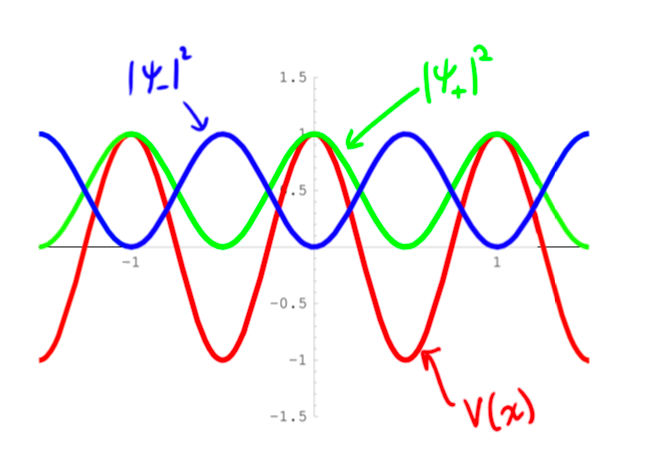
\includegraphics[width=\textwidth]{tb6}
        \caption{Probability amplitudes of diagonalized states, plotted with potential in real-space.}
    \end{figure}
  \item \emph{Case 2}: $\textbf{k}$ near the zone boundary.
  Consider a plane wave $k$ near the zone boundary such that $k = n\pi/a + \delta$. This wavevector  can scatter to
  $k' = -n\pi/a + \delta$. Plugging these wavevectors into the free-energy solution gives unperturbed energies
  $$\epsilon_{0}(k) = \epsilon_{0}(n\pi/a + \delta)) = \frac{\hbar^{2}}{2m}\left [ (n\pi/a)^{2} +2n\pi\delta/a + \delta^{2}\right]$$
  $$\epsilon_{0}(k') = \epsilon_{0}(-n\pi/a + \delta) = \frac{\hbar^{2}}{2m}\left [(n\pi/a)^{2} -2n\pi\delta/a + \delta^{2} \right]$$
  Plugging these into the characteristic equation yields
  $$
  \left (\frac{\hbar^{2}}{2m} \left [(n\pi/a)^{2} + \delta^{2} \right ] - E \right)^{2} = \left ( \frac{\hbar^{2}}{2m} 2n\pi\delta/a\right)^{2} + |V_{G}|^{2}
  $$
  From which we obtain
  $$
  E_{\pm} = \frac{\hbar^{2}((n\pi/a)^{2} + \delta^{2})}{2m} \pm \sqrt{\left (\frac{\hbar^{2}}{2m}2n\pi\delta/a \right )^{2} + |V_{G}|^{2}}
  $$
  If $\delta$ is small, then
  $$
  E_{\pm} \approx \frac{\hbar^{2}(n\pi/a)^{2}}{2m} \pm |V_{G}| + \frac{\hbar^{2}\delta^{2}}{2m}\left [ 1 \pm \frac{\hbar^{2}(n\pi/a)^{2}}{m}\frac{1}{|V_{G}|}\right]
  $$
\end{itemize}
The result of both cases is that we conclude that in the presence of some periodic potential, a gap of size $2|V_{G}|$ opens at the zone boundary and near
the zone boundary this gap is quadratic in $\delta$. See Fig. 7.
\begin{figure}
  \centering
    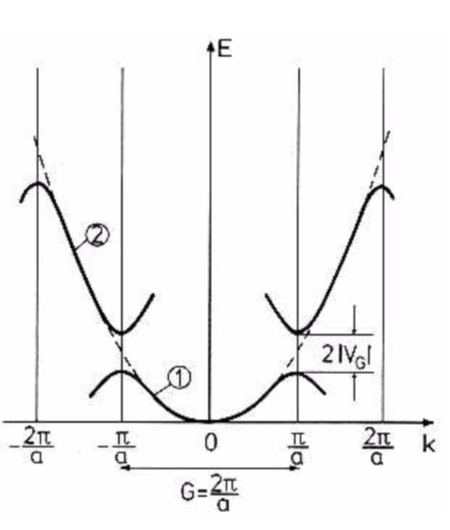
\includegraphics[width=\textwidth]{tb7}
    \caption{Dispersion due to small perturbation in free-electron model.}
\end{figure}
At the Brillouin zone boundaries, the dispersion is parabolic around the extrema of the bands. We can write
$$
E_{+}(G+\delta) = C_{+} + \frac{\hbar^{2}\delta^{2}}{2m^{*}_{+}}
$$
$$
E_{-}(G+\delta) = C_{-} - \frac{\hbar^{2}\delta^{2}}{2m^{*}_{-}}
$$
which gives us the effective masses
$$
m^{*}_{\pm} = \frac{m}{\left |1 \pm \frac{\hbar^{2}(n\pi/a)^{2}}{m}\frac{1}{|V_{G}} \right |}
$$

\subsection{Higher Dimensions}
In two and three dimensions, we observe the following about the nearly free electron model:
\begin{itemize}
  \item Near the Brillouin zone boundary, a gap opens due to scattering by a reciprocal lattice vector.
  \item States of energy slightly higher than the zone boundary are pushed up, while states of energy slightly
  lower are pushed down.
  \item In the one-dimensional case, for $k$ on a zone boundary, there was exactly one $k'$ such that $k' = k + G$
  and $\epsilon_{0(k) = \epsilon_{0}(k')}$. In higher dimensions, there may be multiple $k'$ that may need to be mixed
  to find the degenerate eigenstates. For example, in 2D, $(\pm \pi/a, \pm \pi/a)$ all have the same energy and are separated
  by reciprocal lattice vectors.
\end{itemize}

\section{Bloch's Theorem}
\begin{itemize}
  \item How do we know the plane-wave approach to electrons is valid since the periodic potential may be very strong (and
  therefore, perturbation theory may not be valid)?
  \item No matter how strong the periodic potential, as long as it is periodic, the crystal momentum is conserved.
  \item  \textbf{Bloch's Theorem}: An electron in a periodic potential has eigenstates of the form
  $$\Psi_{\textbf{k}}^{\alpha}(\textbf{r}) = e^{i\textbf{k}\cdot\textbf{r}}u_{\textbf{k}}^{\alpha}(\textbf{r})$$
  where $u_{\textbf{k}}^{\alpha}$ is periodic in the unit cell and the crystal momentum $\textbf{k}$ can be chosen
  within the first Brillouin zone.
  \item There may be many states at each $\textbf{k}$ and these are indexed by $\alpha$.
  \item The function $u$ is known as the \emph{Bloch function} and $\Psi$ is sometimes called the \emph{modified plane wave}.
  \item Because $u$ is periodic in the unit cell, we can write
  $$
  u_{\textbf{k}}^{\alpha}(\textbf{r}) = \sum_{\textbf{G}} \tilde{u}_{\textbf{G},\textbf{k}}^{\alpha}(\textbf{r})e^{i\textbf{G}\cdot\textbf{r}}
  $$
  which guarantees that $u_{\textbf{k}}^{\alpha}(\textbf{r}) = u_{\textbf{k}}^{\alpha}(\textbf{r} + \textbf{R})$.
  \item The modified plane wave can then be written as
  $$\Psi_{\textbf{k}}^{\alpha}(\textbf{r}) = \sum_{\textbf{G}} \tilde{u}_{\textbf{G},\textbf{k}}^{\alpha}(\textbf{r})e^{i(\textbf{G}+\textbf{k})\cdot\textbf{r}}$$
  REVISIT TO FINISH.
\end{itemize}
To do: Chapters 15, 16, 23, 17
\end{document}
